\documentclass{article}
\usepackage[utf8]{inputenc}
\usepackage{listings}
\usepackage{geometry}
\usepackage{graphicx}

\graphicspath{.}
\title{COMP1204 Data management: Coursework 2}
\author{Kritagya Gurung}

\begin{document}
	
	\maketitle
	\begin{center}
		Student ID: 30220238
	\end{center}
	
	\newpage

	\section{The Relational Model}

	\subsection{EX1}
	
	\begin{center}
		\begin{tabular}{||c c | c c | c c ||} 
			\hline
			Attribute name & data type & Attribute name & data type & Attribute name & data type \\
			\hline
			Hotel ID & int & Overall rating & float & Avg. Price & int \\ 
			URL & string & Author & string & Content & string \\ 
			Date & string & No. Reader & int & No. Helpful & int \\ 
			Overall & int & Value & int & Rooms & int \\
			Location & int & Cleanliness & int & Check in/Front desk & int \\
			Service & int & Business service & int &  &  \\
			\hline
		\end{tabular}
	\end{center}
	Relation Schema: 
	\newline
	(R1)Review(Hotel ID, Overall rating, Avg. Price, URL, Author, Content, Date, No. Reader, No. Helpful, Overall, Value, Rooms, Location, Cleanliness, Check in/Front desk, Service, Business service).
	\newline
	The primary key consists of Hotel ID, Author and date. This is because all other attributes rely on the attributes mentioned and in order to write a review, you must have an author, the date that review was written on and what hotel the review is for.
		
	\subsection{EX2}
	\begin{math}
		\textrm{Hotel ID}
		\rightarrow
		\textrm{Overall rating, Avg. Price, URL}
	\end{math}
	\newline
	Hotel ID is the determinant for Overall rating, Avg. Price and URL. This is because each hotel has their own distinct properties.
	\newline
	\begin{math}
		\textrm{Author, Date}
		\rightarrow
	\end{math}
	Content, No. Reader, No. Helpful, Overall, Value, Rooms, Location, Cleanliness, Check in/Front desk, Service, Business service.
	\newline
	Author and Date should be the determinant for all other attributes since it is the author who decides the scores and the content of the review on a hotel. Additionally, the author must stay at the hotel thus date is used to show when the hotel was reviewed.
	\newline
	Candidate keys:
	\newline
	Hotel ID, Author, Date
	\subsection{EX3}
	\begin{center}
		\begin{tabular}{||c c | c c | c c ||} 
			\hline
			Attribute name & data type & Attribute name & data type & Attribute name & data type \\
			\hline
			Hotel ID & int & Overall rating & float & Avg. Price & int \\ 
			URL & string & Author & string & Content & string \\ 
			Date & string & No. Reader & int & No. Helpful & int \\ 
			Overall & int & Value & int & Rooms & int \\
			Location & int & Cleanliness & int & Check in/Front desk & int \\
			Service & int & Business service & int & User ID & int \\
			\hline
		\end{tabular}
	\end{center}
	Hotel(Hotel ID, Avg. Price, Date) \\
	Review(Hotel ID, User ID, Content, Date, No. Reader, No. Helpful, Overall, Value, Rooms, Location, Cleanliness, Check in/Front desk, Service, Business service) \\
	Author(User ID, Author) \\
	Primary Key : Hotel ID, User ID, Date \\
	Foreign Key : Hotel ID, User ID \\
	
	\section{Entity-Relationship Diagramming}
	
	\subsection{EX4}
	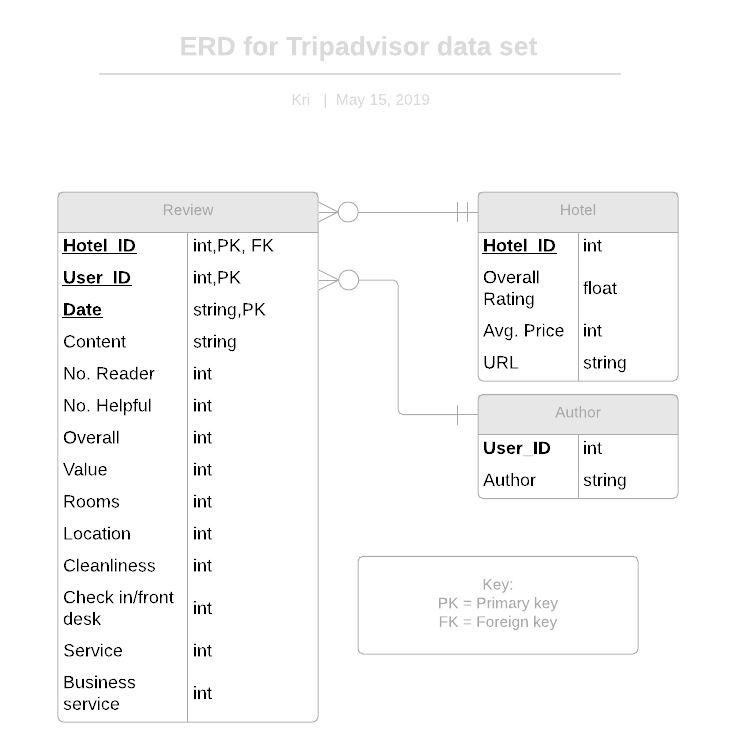
\includegraphics[width=10cm, height=10cm]{EX4_ERD_Tripadvisor.png}
	
	
	\section{Relational Algebra}
	
	\subsection{EX5}
	\begin{eqnarray}
	\sigma_{User\_ID = given\_ID}(Review)
	\end{eqnarray}
		
	\subsection{EX6}
	\begin{eqnarray}
	\sigma _{No. reviews given > 2}(_{User\_ID} \gamma _{count(User\_ID) \rightarrow No. reviews given}(Review)) \bowtie Author
	\end{eqnarray}
	
	\subsection{EX7}
	\begin{eqnarray}
		\sigma _{No. reviews received > 10}(_{Hotel\_ID} \gamma _{count(Hotel\_ID) \rightarrow No. reviews received}(Review))
	\end{eqnarray}
	
	\subsection{EX8}
	\begin{eqnarray}
	\sigma _{Average cleanliness \geq 4.5 \wedge Overall rating > 3}((_{Hotel\_ID} \gamma _{avg(Cleanliness) \rightarrow Average cleanliness}(Review)) \bowtie (Hotel))
	\end{eqnarray}
	
	\section{SQL Queries}
	
	\subsection{EX9}
	CREATE TABLE HotelReviews(
	Hotel\_ID INTEGER,
	Overall\_rating REAL,
	Average\_price INTEGER,
	URL TEXT,
	Author TEXT,
	Content TEXT,
	Date TEXT,
	Number\_of\_readers INTEGER,
	Number\_of\_helpful INTEGER,
	Overall INTEGER,
	Value INTEGER,
	Rooms INTEGER,
	Location INTEGER,
	Cleanliness INTEGER,
	Check\_in\_and\_Front\_desk INTEGER,
	Service INTEGER,
	Business\_service INTEGER,
	PRIMARY KEY(Hotel\_ID, Author, Date)
	);
	
	\subsection{EX10}
	Bash scripting not available.
	
	\subsection{EX11}
	CREATE TABLE Hotel (
	Hotel\_ID INTEGER PRIMARY KEY,
	Overall\_rating REAL,
	Average\_price INTEGER,
	URL TEXT
	); 
	\\
	CREATE TABLE Author (
	User\_ID INTEGER PRIMARY KEY,
	Author TEXT
	);	
	\\
	CREATE TABLE Review (
	Hotel\_ID INTEGER,
	User\_ID TEXT,
	Content TEXT,
	Date TEXT,
	Number\_of\_readers INTEGER,
	Number\_of\_helpful INTEGER,
	Overall INTEGER,
	Value INTEGER,
	Rooms INTEGER,
	Location INTEGER,
	Cleanliness INTEGER,
	Check\_in\_and\_Front\_desk INTEGER,
	Service INTEGER,
	Business\_service INTEGER,
	FOREIGN KEY (Hotel\_ID) REFERENCES Hotel(Hotel\_ID),
	FOREIGN KEY (User\_ID) REFERENCES Author(User\_ID),
	PRIMARY KEY (Hotel\_ID,User\_ID,Date)
	);
	
	
	\subsection{EX12}
	As the bash scripting does not work as intented, I have made my custom test data.
	Here is the test data set I used.
	INSERT INTO Hotel(Hotel\_ID,Overall\_rating,Average\_price,URL)
	VALUES(11111,2.0,13,"test url1"),
	(11112,4,123,"test url2");
	\\
	INSERT INTO Author(User\_ID,Author)
	VALUES(1,"testAuthor1"),
	(2,"testAuthor2"),
	(3,"testAuthor3");
	\\
	INSERT INTO Review(Hotel\_ID, User\_ID, Content, Date,Number\_of\_readers, Number\_of\_helpful, Overall, Value, Rooms, Location, Cleanliness, Check\_in\_From\_desk, Service, Business\_service)
	VALUES(11111,1,"contentTest","dateTest",1,2,3,4,5,6,7,8,9,10),
	(11112,2,"contentTest","dateTest",1,2,3,4,5,6,7,8,9,10),
	(11111,3,"contentTest","dateTest",1,2,3,4,5,6,7,8,9,10),
	(11112,2,"contentTest","dateTest2",1,2,3,4,5,6,7,8,9,10),
	(11111,2,"contentTest","dateTest",1,2,3,4,5,6,7,8,9,10),
	(11112,3,"contentTest","dateTest",1,2,3,4,5,6,7,8,9,10),
	(11112,3,"contentTest","dateTest2",1,2,3,4,5,6,7,8,9,10),
	(11112,3,"contentTest","dateTest3",1,2,3,4,5,6,7,8,9,10),
	(11112,3,"contentTest","dateTest4",1,2,3,4,5,6,3,8,9,10),
	(11112,3,"contentTest","dateTest5",1,2,3,4,5,6,7,8,9,10),
	(11112,3,"contentTest","dateTest6",1,2,3,4,5,6,7,8,9,10),
	(11112,3,"contentTest","dateTest7",1,2,3,4,5,6,3,8,9,10),
	(11112,3,"contentTest","dateTest8",1,2,3,4,5,6,7,8,9,10),
	(11112,3,"contentTest","dateTest9",1,2,3,4,5,6,7,8,9,10),
	(11112,3,"contentTest","dateTest10",1,2,3,4,5,6,7,8,9,10),
	(11112,3,"contentTest","dateTest11",1,2,3,4,5,6,3,8,9,10);
	\\
	DROP TABLE IF EXISTS HotelReviews;
	
	
	\subsection{EX13}
	I would have added indexes to Hotel\_ID and User\_ID attributes as they are used as the main attributes in table joins, they are used in multiple queries and are foreign keys. \\
	CREATE INDEX Hotel\_ID\_Index ON Hotel(Hotel\_ID); \\
	CREATE INDEX User\_ID\_Index ON Author(User\_ID);
	
	\subsection{EX14}
	\textbf{ex5.sql} \\
	SELECT  * FROM Review WHERE User\_ID=2;
	\\
	(replace 2 with a given id)
	\\
	\textbf{ex6.sql} \\
	SELECT Hotel\_ID,count(*) AS Number\_of\_reviews\_recieved
	FROM Review
	GROUP BY Hotel\_ID HAVING count(*); 
	\begin{math}
	>
	\end{math} 
	10;
	\\
	\textbf{ex7.sql} \\
	SELECT Review.User\_ID,Author.Author , count(*) AS Number\_of\_reviews\_given
	FROM Review INNER JOIN Author ON Author.User\_ID = Review.User\_ID 
	GROUP BY Review.User\_ID HAVING count(*) 
	\begin{math}
	>
	\end{math} 
	2;
	\\
	\textbf{ex8.sql} \\
	SELECT Review.Hotel\_ID, Hotel.Overall\_rating, Hotel.Average\_price, Hotel.URL , avg(Review.Cleanliness) AS Average\_cleanliness
	FROM Review INNER JOIN Hotel ON Review.Hotel\_ID = Hotel.Hotel\_ID 
	GROUP BY Review.Hotel\_ID HAVING Average\_cleanliness 
	\begin{math}
	\geq
	\end{math}
	 4.5 AND Overall\_rating 
	 \begin{math}
	 >
	 \end{math}
	 3;
	
	\section{Conclusions}
	
	\subsection{EX15}
	

\end{document}